\section{Classification} \label{sec:classfication}

\begin{figure*}
    \centering
    \fbox{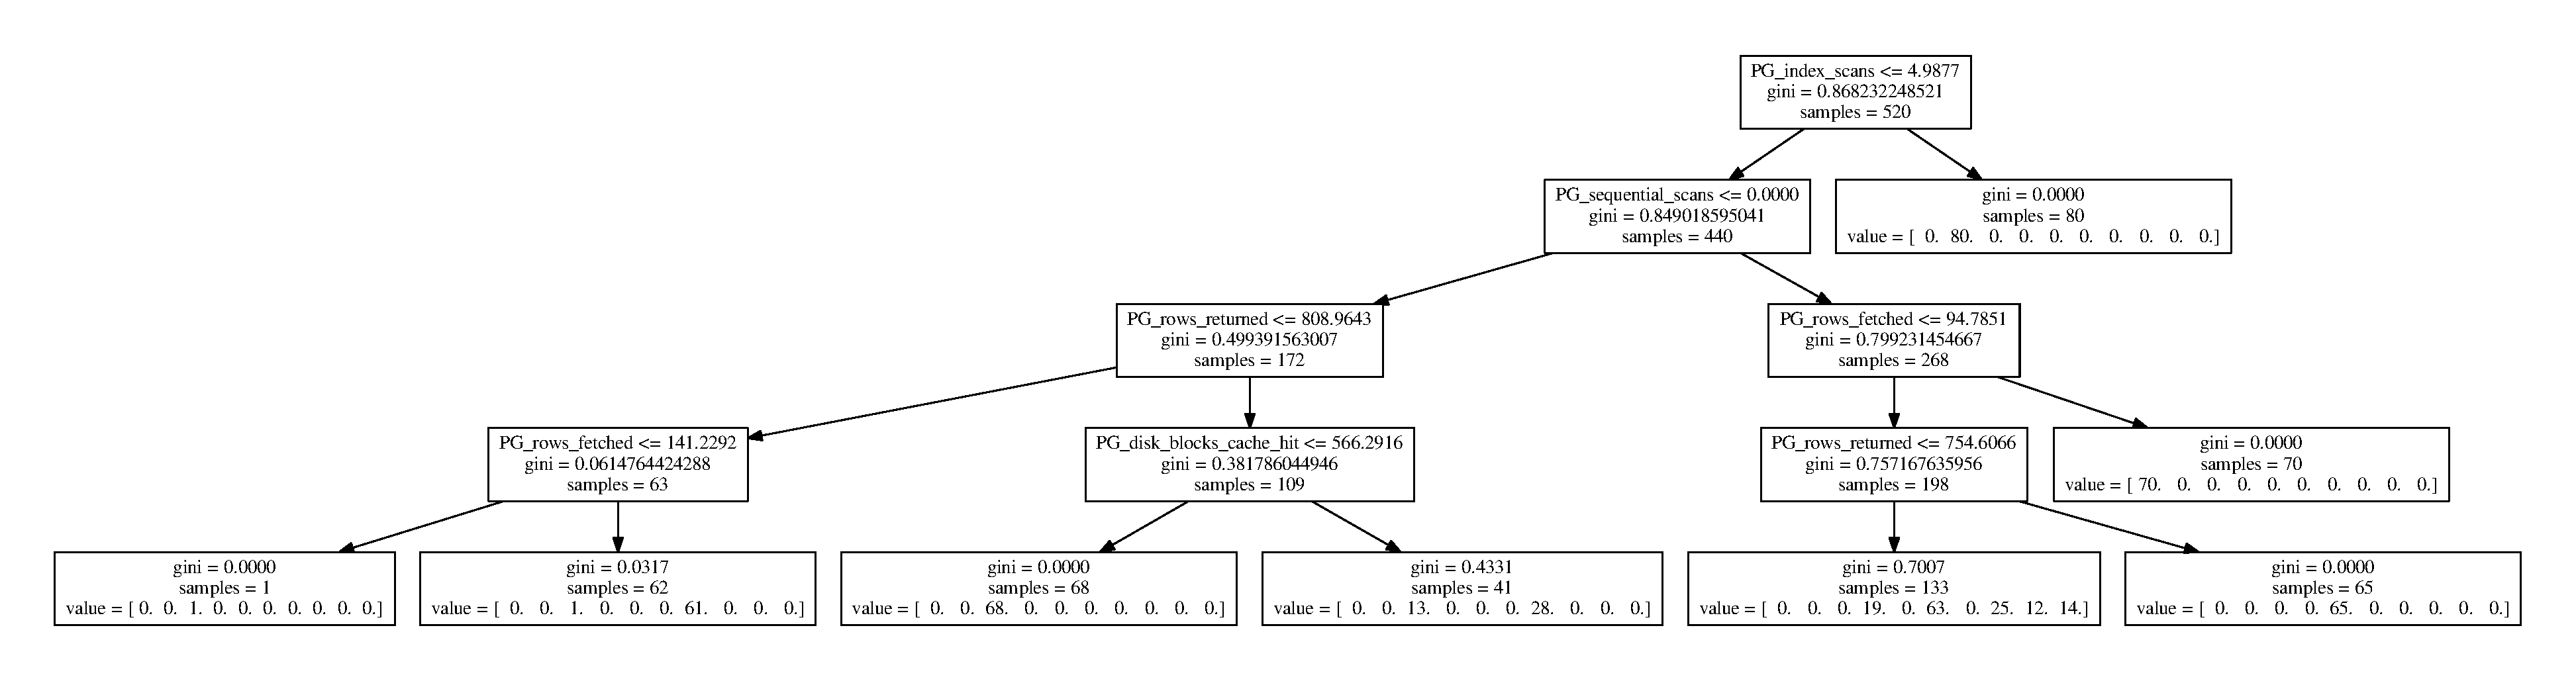
\includegraphics[width=\linewidth]{figure/tree_4.pdf}}
    \caption{Decision tree with max depth set to 4.}
    \label{fig:tree_4}
\end{figure*}

\begin{figure*}
    \centering
    \fbox{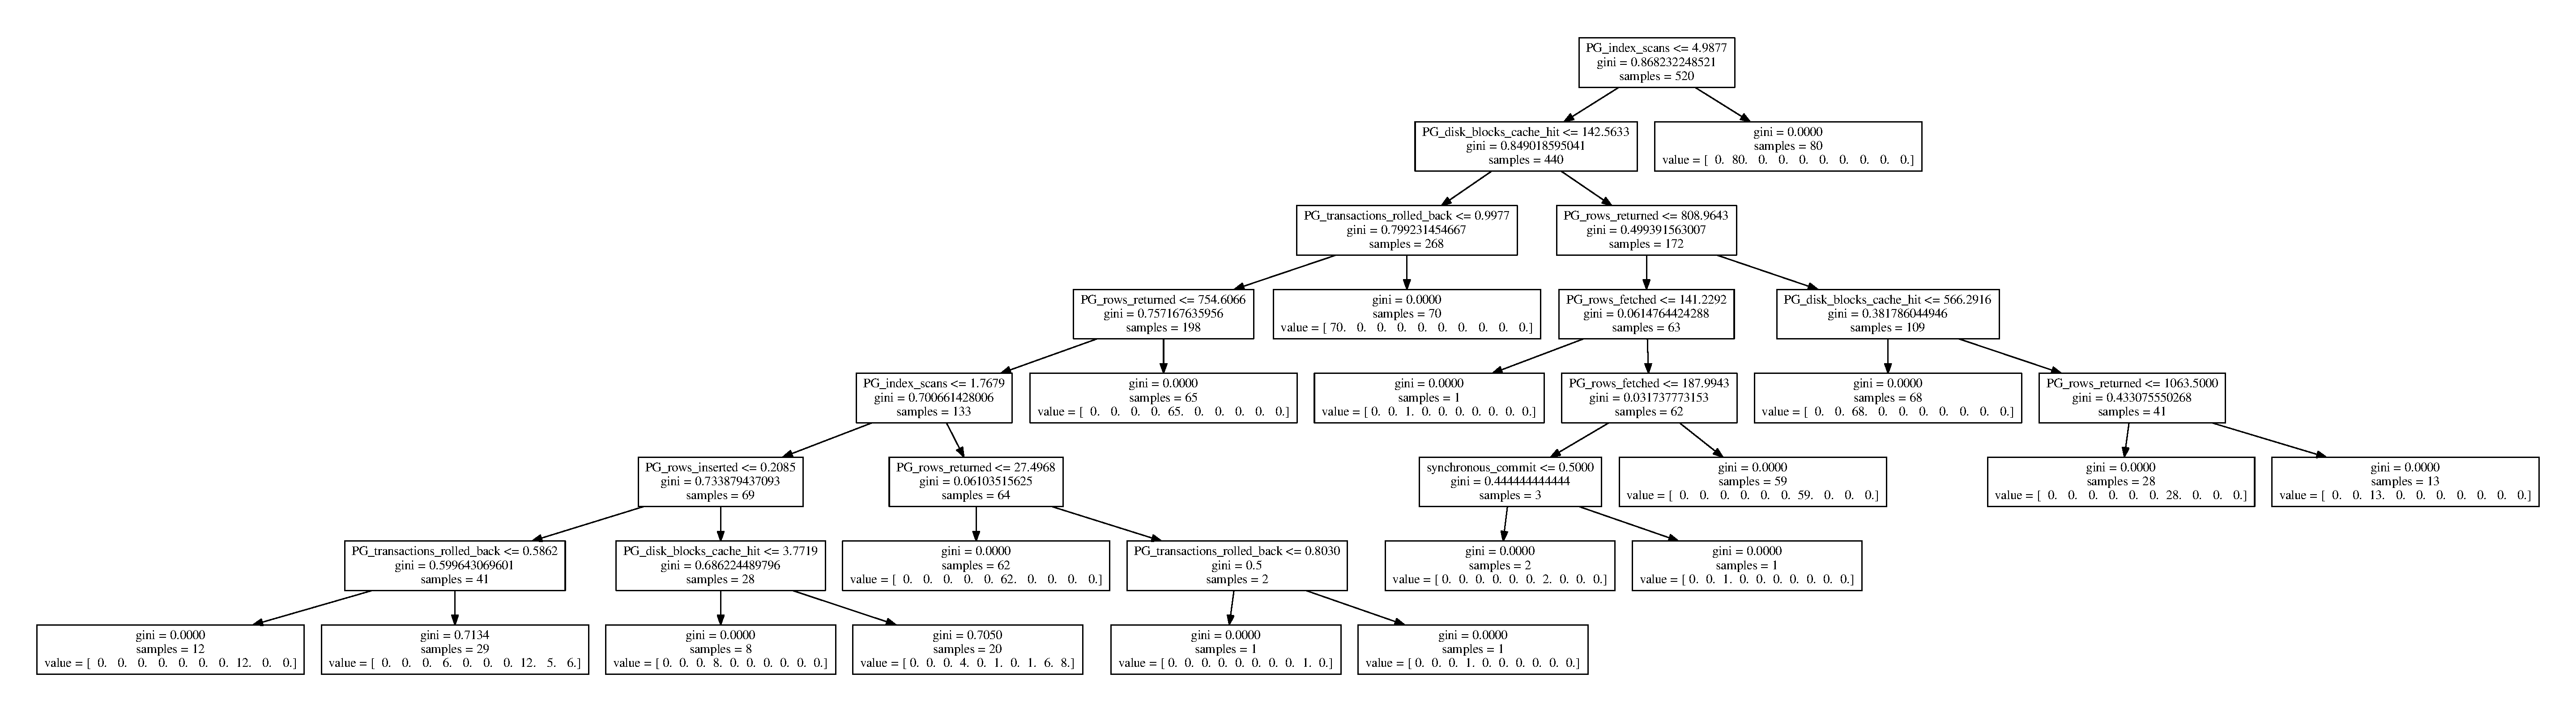
\includegraphics[width=\linewidth]{figure/tree_7.pdf}}
    \caption{Decision tree with max depth set to 7.}
    \label{fig:tree_7}
\end{figure*}

\begin{figure*}
    \centering
	\subfloat[\label{fig:dt_depth}]{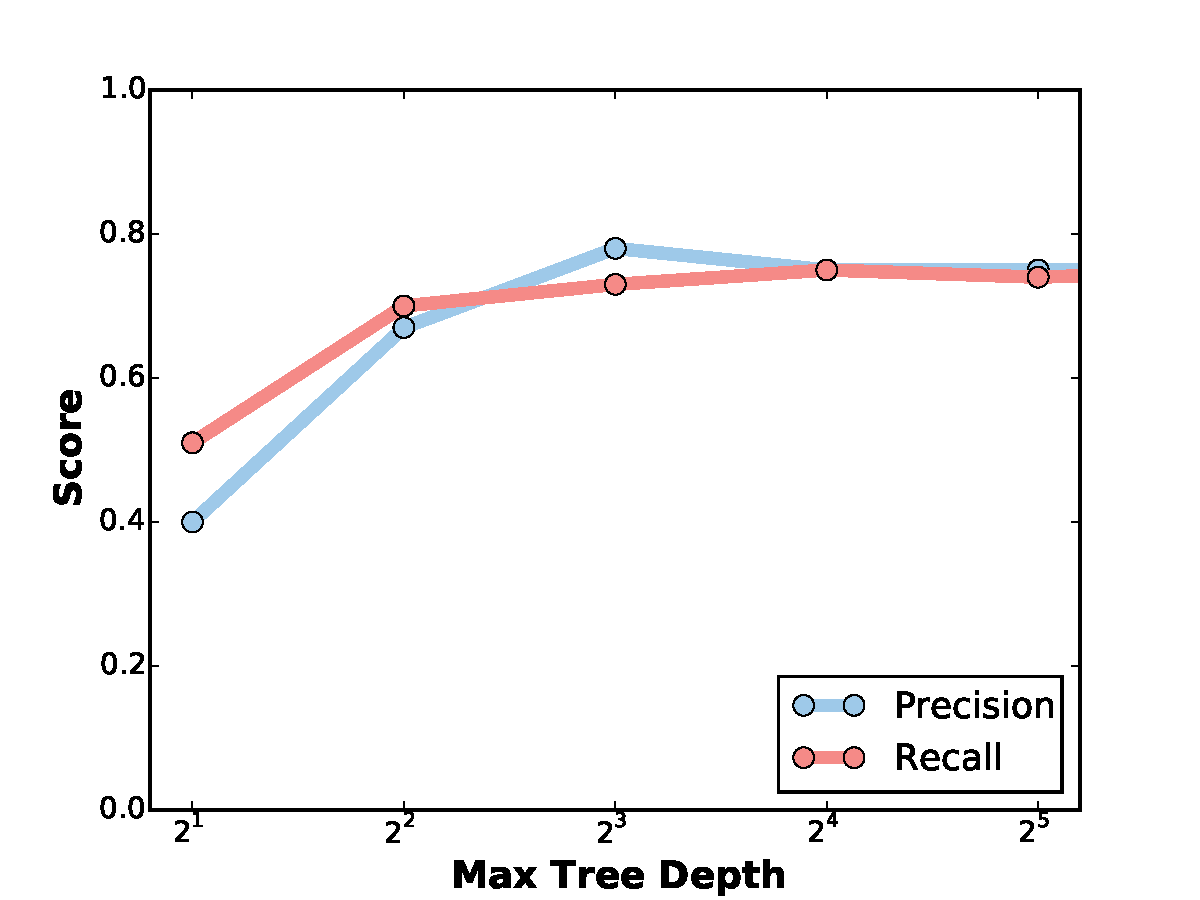
\includegraphics[width=0.4\linewidth]{figure/depth.pdf}}
	\subfloat[\label{fig:dt_leaves}]{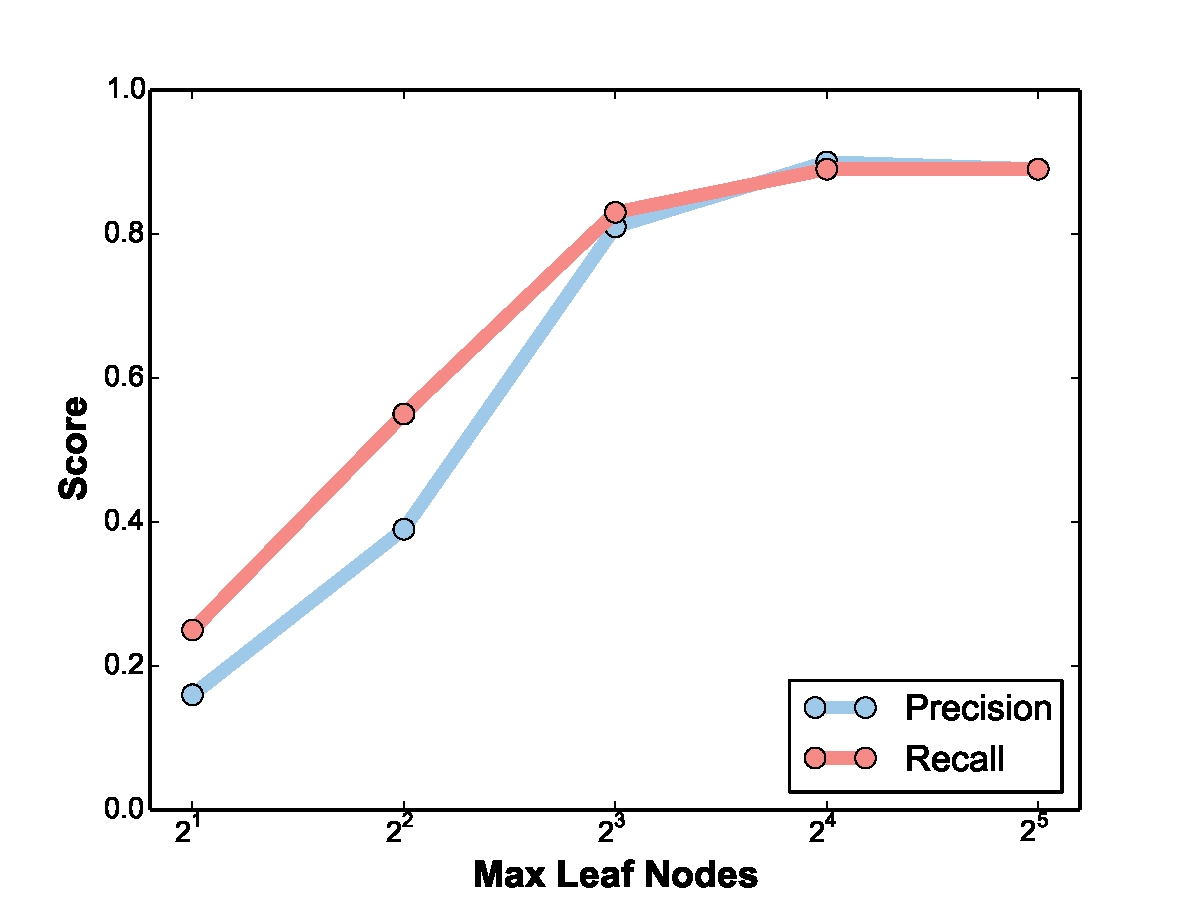
\includegraphics[width=0.4\linewidth]{figure/leaves.pdf}}
	\caption{Impact of max depth and max leaf nodes on the accuracy of the
    decision tree.}
\end{figure*}

\begin{table}
\centering
\small{
  \centering
  \begin{tabular}{l|llll} 
	\toprule
   		Class &  Precision  &  Recall &  F1-score  &  Support  \\    
    \midrule
		0.0   &    1.00   &   0.00   &   1.00   &     84   \\
        1.0   &    0.99   &   1.00   &   0.99   &     74   \\
        2.0   &    0.98   &   0.99   &   0.98   &     81   \\
        3.0   &    0.54   &   0.39   &   0.45   &     18   \\
        4.0   &    1.00   &   1.00   &   1.00   &     69   \\
        5.0   &    1.00   &   0.99   &   0.99   &     70   \\
        6.0   &    1.00   &   0.95   &   0.97   &     60   \\
        7.0   &    0.41   &   0.95   &   0.57   &     19   \\
        8.0   &    0.00   &   0.00   &   0.00   &     17   \\
        9.0   &    0.56   &   0.52   &   0.54   &     27   \\
    \midrule
Avg / Total   &    0.90   &   0.91   &   0.90   &    519   \\
   \bottomrule&
   \end{tabular}
 }
%\nocaptionrule
\caption{Per-class accuracy of the default decision tree.}
\label{tab:dt_stats}
\end{table}


% -----------------------------------------------
% Estimated number of clusters: 10
% Homogeneity: 0.614
% Completeness: 0.628
% V-measure: 0.621
% Adjusted Rand Index: 0.429
% Adjusted Mutual Information: 0.606
% [2 8 9 ..., 3 1 1]
% Silhouette Coefficient: 0.111
% 
% Metrics for Affinity Propogation
% -----------------------------------------------
% Estimated number of clusters: 88
% Homogeneity: 0.654
% Completeness: 0.317
% V-measure: 0.427
% Adjusted Rand Index: 0.067
% Adjusted Mutual Information: 0.248
% [72  8 22 ..., 30 74 39]
% Silhouette Coefficient: 0.082
% 
% Metrics for Mean-Shift
% -----------------------------------------------
% Estimated number of clusters: 2
% Homogeneity: 0.012
% Completeness: 0.368
% V-measure: 0.024
% Adjusted Rand Index: -0.001
% Adjusted Mutual Information: 0.010
% [0 0 0 ..., 0 0 0]
% Silhouette Coefficient: 0.517
% 
% Metrics for Ward Agglomerative Clustering
% -----------------------------------------------
% Estimated number of clusters: 10
% Homogeneity: 0.589
% Completeness: 0.635
% V-measure: 0.611
% Adjusted Rand Index: 0.458
% Adjusted Mutual Information: 0.581
% [0 4 5 ..., 4 2 6]
% Silhouette Coefficient: 0.097
